\documentclass[twoside]{article}
\usepackage{graphicx}
\usepackage{polski}
\usepackage{fancyhdr}
\usepackage{lastpage}
\usepackage{listings}
\usepackage{soul}
\usepackage{color}
\usepackage{multirow}
\usepackage{subcaption}
\usepackage{fancyvrb}


\title{AiSD Ex. 2 (Pon.)}
\author{\hl{Mateusz Kamieniecki}}
\date{\today}

\lstset{
    numbers=left
}

\makeatletter

\begin{document}

\pagestyle{fancy}
\fancyhead{}
\fancyhead[L]{\@title}
\fancyhead[R]{\@author}
\fancyhead[C]{\@date}

\cfoot{\thepage\ / \pageref{LastPage}}


\newpage

\section{Wprowadzenie}
Praca ,,na danych'' oznacza konieczność wykorzystywania danych, co może przykładowo przejawiać
się w ich: przenoszeniu z jednego punktu do drugiego, powielaniu, modyfikowaniu, filtrowaniu, porządkowaniu, przeszukiwaniu.

Formą porządkowania danych może być ich posortowanie, a to już umiemy zrobić (po wykonaniu pierwszego ćwiczenia).
Wiemy również, że problem sortowania nie ma jednego rozwiązania, a ich
mnogość zależy od wielu czynników (rodzaju danych, wielkości porządkowanej kolekcji, dostępności zasobów (zarówno sprzętowych jak i ludzkich) oraz bibliotek).

Powinniśmy już mieć również świadomość w jaki sposób możemy przeszukiwać kolekcję pod kątem
występowania w niej określonego elementu.
W przypadku nieuporządkowanej (nieposortowanej) kolekcji jesteśmy ograniczeni przez podejście
naiwne (liniowe; sekwencyjne), czyli stosując \textbf{algorytm wyszukiwania sekwencyjnego} 
(rys. \ref{fig:linear-search-label}) przechodzimy od początku do końca kolekcji sprawdzając 
element po elemencie dopasowanie do wyszukiwanej wartości.
Niewątpliwą zaletą tego podejścia jest to, że działa ono dla \underline{nieuporządkowanego} zestawu wartości.
Wadą natomiast jest złożoność takiego przeszukiwania, które charakteryzuje się złożonością liniową
($O(n)$).

\begin{figure}[h]
    \centering
    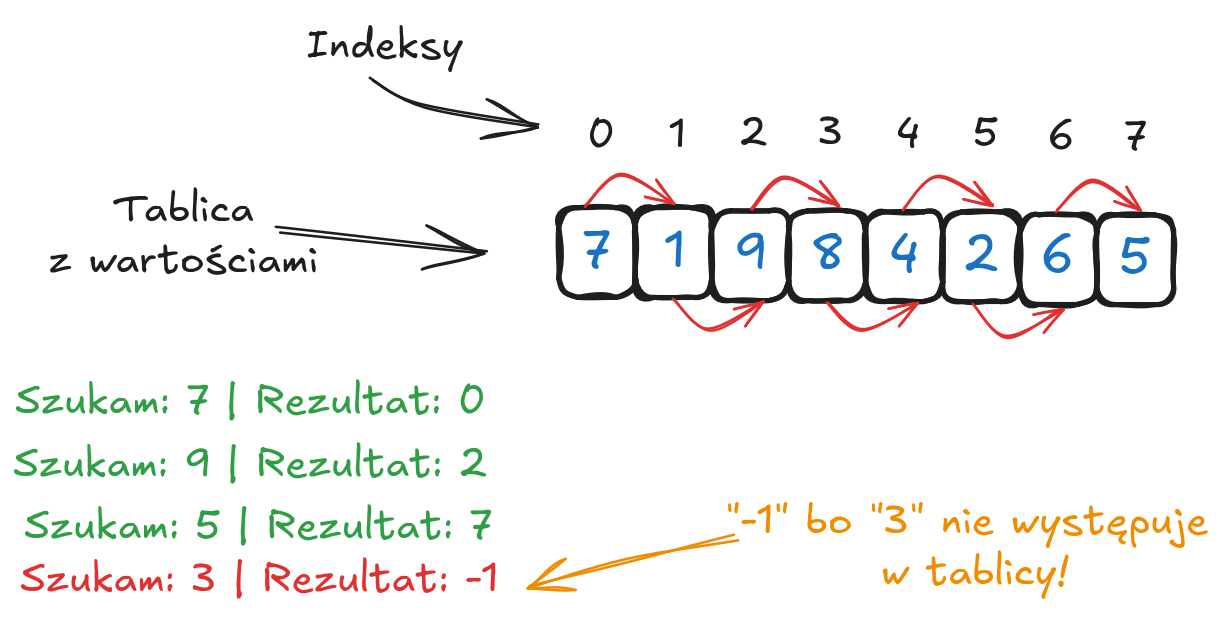
\includegraphics[width=0.75\linewidth]{images/1_linear_search.png}
    \caption{Wizualizacja algorytmu przeszukiwania liniowego. 
    Mamy nieuporządkowaną kolekcję ośmiu elementów, którą przechodzimy od lewej (indeks 0)
    do prawej (indeks 7). Jeśli poszukiwany element znajduje się w tablicy, to zwracamy indeks,
    pod którym występuje. W przeciwnym razie zwracamy (umownie):~-1.}
    \label{fig:linear-search-label}
\end{figure}

Alternatywnym pomysłem, gdy mamy \underline{uporządkowaną} (posortowaną) kolekcję, jest użycie
\textbf{algorytmu wyszukiwania binarnego} opierającego się na podejściu \textit{dziel i zwyciężaj}.
Pierwsze spotkanie z tym problemem mieliśmy w~trakcie zajęć wprowadzających, dlatego nie będziemy
teraz ponownie szczegółowo analizowali tego problemu. Trzeba jednak odnotować, że uzyskiwane
rezultaty działania tego algorytmu powinny być identyczne jak w przypadku naiwnym, czyli zwracamy
indeks tablicy, pod którym występuje poszukiwana wartość, lub \verb|-1|, jeśli wartość 
nie występuje w kolekcji.

Złożoność wyszukiwania (binarnego) elementu pośród n-elementowej tablicy jest określana jako
$O(\log(n))$, a wynika to z tego, że dla przykładowego $n=100$ zwrócenie wyniku powinno nastąpić
po maksymalnie $\lfloor log_2(100) + 1 \rfloor = 7$ iteracjach pętli porównującej wyszukiwaną
wartość i~poławiającej (dzielącej na ,,połowę'') przeszukiwany zakres.

Czy można to sobie jakoś lepiej zwizualizować? Można!
Proszę narysować zrównoważone drzewo poszukiwań binarnych reprezentujące naszą uporządkowaną kolekcję, a następnie proszę sprawdzić, ile porównań trzeba wykonać, żeby dojść do elementu
znajdującego się na najniższym poziomie w drzewie.

Bezdyskusyjnie algorytm wyszukiwania binarnego (dla uporządkowanej kolekcji) bije na głowę
algorytm liniowy. Jest to tym bardziej zauważalne, im większa jest liczba elementów w kolekcji.
A teorię \underline{($O(\log (n) < O(n)$)} można bez problemu potwierdzić praktycznym przykładem.

Pojawia się jednak dodatkowe pytanie: \textbf{czy można szybciej}?
Czy można uniezależnić czas wyszukiwania elementu od wielkości kolekcji?

Odważmy się i postawmy to pytanie! Czy można osiągnąć stałą złożoność ($O(1)$)?
I teraz, od razu, idąc na skróty, odpowiedzmy: można!

\subsection{Adresowanie bezpośrednie}
Można stworzyć kolekcję, która będzie miała stałą ($O(1)$) złożoność dla operacji wyszukiwania
elementów.
Ale dodatkowo ta kolekcja może mieć taką samą (stałą) złożoność dla operacji dodawania i usuwania
elementów.
Brzmi zaskakująco? To spróbujmy rzucić na ten tajemniczy problem nieco światła.

Jednym z pomysłów na to zagadnienie jest wykorzystanie \textbf{adresowania bezpośredniego}.
Wyobraźmy sobie, że każdy element, który chcemy przechowywać, da się jednoznacznie odwzorować na unikalną liczbę całkowitą, którą na potrzeby tego rozważania będziemy nazywać kluczem.
Jeżeli jesteśmy w stanie określić, że nasze klucze \verb|key| są z zakresu $key \in <0; m-1>$, 
a $m$ nie jest zbyt dużą wartością, to możemy wszystkie nasze elementy umieścić w tablicy
$T[0... m-1]$.
Wyszukanie elementu będzie wymagało od nas jedynie wyliczenia wartości klucza \verb|key| i sprawdzenia, czy w tablicy $T$ pod danym indeksem jest wartość inna niż \verb|null| 
(\verb|T[key] == null|).

Wstawianie elementu będzie przeprowadzane poprzez zastąpienie w tablicy $T$ pod indeksem $key$ wartości \verb|null| wstawianym elementem (czyli: \verb|T[key] =| \verb|element|).
A usunięcie będzie wyglądało analogicznie (po wyliczeniu klucza dla wartości, której chcemy się pozbyć z kolekcji): \verb|T[key] = null|.

Istotną wadą tego pomysłu jest założenie, że nasze klucze muszą być mniejsze od niezbyt dużego $m$ ($key < m$). Dlaczego mamy takie ograniczenie? Ponieważ $m$ określa nam rozmiar tablicy \verb|T|,
a w pamięci komputera nie możemy dysponować nieograniczoną pamięcią.

Dodatkową wadą jest fakt, że nawet jeśli naszych wartości nie będzie zbyt wiele, ale ich 
odwzorowanie na klucze będzie generowało duże wartości (czyli: $n=100$, $max\_key=1\_000\_000$),
to stosując podejście adresowania bezpośredniego zaalokujemy tablicę o rozmiarze $1\_000\_000$,
a $999\_900$ jej komórek będzie wypełnionych wartością $null$ ($99.99\%$ komórek tabeli będzie
niewykorzystanych).

Jak widzimy, adresowanie bezpośrednie jest stosunkowo prostym zagadnieniem, ale nadaje się
bardziej do rozważań teoretycznych niż praktycznych zastosowań w codziennych, typowych
(programistycznych) zadaniach.

\subsection{Tablica z haszowaniem}
Wymienione wady adresowania bezpośredniego nie zachęcają do wykorzystywania go w praktycznych 
zastosowaniach.
Nie przekreślają one jednak samej idei, którą wystarczy trochę zmodyfikować, aby uzyskać rozwiązanie
znacznie bardziej nadające się do użytku nie tylko na polu akademickim ale również w~świecie
komercyjnym.

Tym ,,ulepszeniem'' jest \textbf{tablica z haszowaniem} (tablica mieszająca).
Zobaczyliśmy, że w adresowaniu bezpośrednim element zmapowany na klucz \verb|key| jest umieszczony
w~tablicy \verb|T| pod indeksem \verb|key| (\verb|T[key] = | \verb|element|). 
A~w~przypadku tablicy z haszowaniem $T_H$ nasz element trafia pod indeks wyliczony przez 
\textbf{funkcję haszującą} (funkcję mieszającą) $h(key)$, czyli \verb|T[h(key)] = element|.

Ideą tej funkcji $h(key)$ jest odwzorowanie klucza \verb|key| na indeks tablicy $T_H[0...m-1]$, 
gdzie $m$ jest rozmiarem tablicy z haszowaniem, który zazwyczaj jest znacznie mniejszy
od \verb|max_key| (czyli największej wartości z uniwersum wszystkich kluczy).
Wypada zauważyć, że wartość wyliczona przez funkcję $h(key)$ jest nazywana 
\textbf{wartością haszującą} klucza $key$.

Jeśli w ten sposób redukujemy rozmiar tablicy $T_H$ (w porównaniu do adresowania bezpośredniego), 
to tym samym zmniejszamy liczbę pustych, nieużywanych indeksów tablicy (wypełnionych przez
\verb|null|).

Wobec powyższego powstaje oczekiwanie, że funkcja haszująca $h(key)$ będzie dobrze rozpraszała
wartości po tablicy unikając powtórzeń wyliczonych indeksów.

Należy sobie teraz postawić pytanie: co zrobimy, jeżeli to oczekiwanie nie zostanie spełnione?
Co zrobimy, jeśli dla dwóch różnych elementów zostaną wyliczone dwa różne unikalne klucze 
$key_1, key_2$, ale dla tych dwóch różnych kluczy funkcja haszująca $h(key)$ zwróci 
taką samą wartość haszującą ($key_1 \neq key_2, h(key_1) = h(key_2)$)?

Taką sytuację -- sytuację, gdy dla dwóch różnych kluczy wyliczamy takie same wartości haszujące --
nazywamy \textbf{kolizją}.
Podobnie jak w życiu tak i w programowaniu wolimy (a przynajmniej powinniśmy woleć, jeśli nie mamy
skłonności masochistycznych) unikać kolizji.
Niestety te kolizje czasami występują, dlatego warto ustalić, co możemy zrobić w takiej sytuacji.

Jednym z pomysłów (i na tym koncentrujemy się w tym ćwiczeniu) jest \textbf{rozwiązanie kolizji
metodą łańcuchową} (rys. \ref{fig:hash-linear-probing-label}), co oznacza, że w tablicy mieszającej
$T_H$ pod indeksem wyliczonym przez funkcję haszującą jest lista liniowa, którą wypełniamy
elementami o tej samej wartości haszującej.

\begin{figure}[ht]
    % \centering
    \centerline{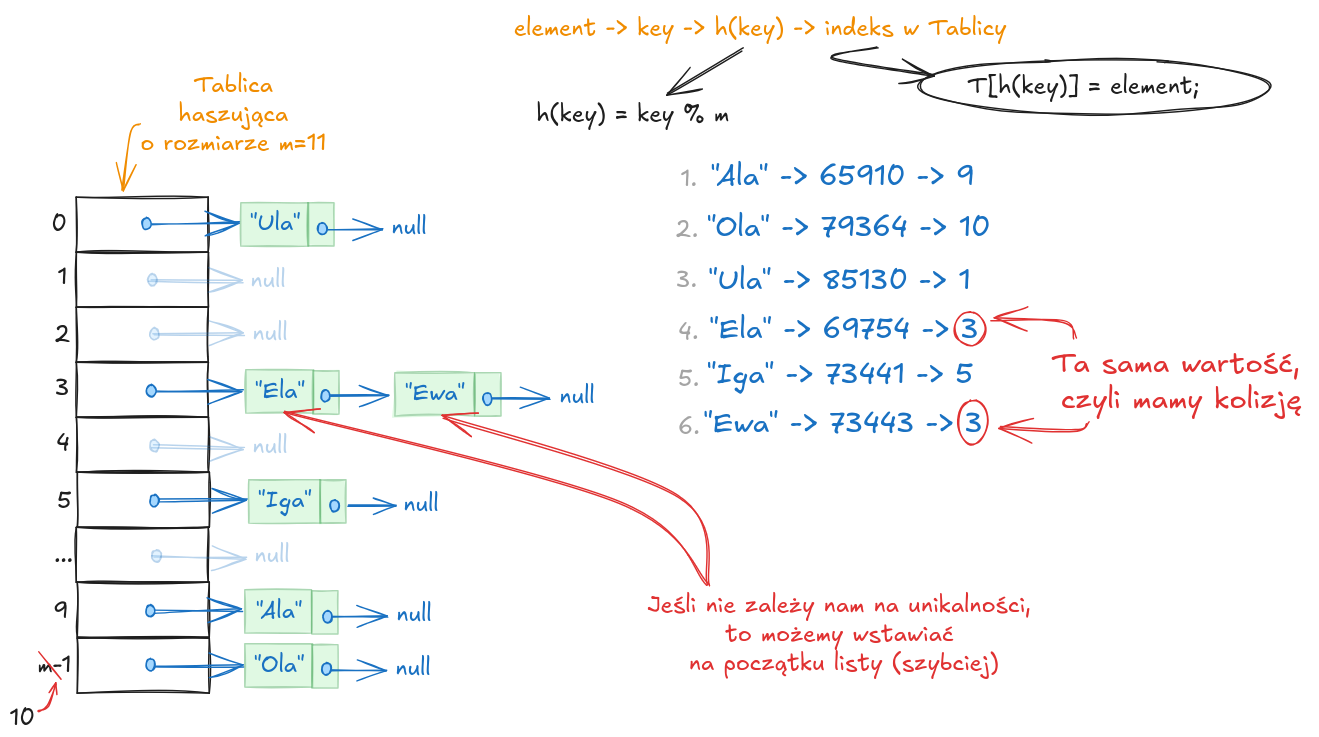
\includegraphics[width=1.4\linewidth]{images/2_hash_linear_probing.png}}
    \caption{Przykład tablicy mieszającej (o rozmiarze m=11) z rozwiązywaniem kolizji metodą
    łańcuchową. Doszło do kolizji dla elementów "Ela" oraz "Ewa" -- obydwa otrzymały taką samą
    wartość z funkcji haszującej. Wybraną funkcją haszującą było haszowanie modularne.}
    \label{fig:hash-linear-probing-label}
\end{figure}

Dla tablicy haszującej możemy wprowadzić \textbf{współczynnik zapełnienia $\alpha$ tabeli} $T_H$, taki że:
$$\alpha=\frac{n}{m}$$
, gdzie $n$ jest liczbą elementów w tablicy, a $m$ jest rozmiarem tablicy.

Przyjmuje się, że dla $\alpha < 0.75$ tablica mieszająca będzie działała sprawnie
(złożoność $O(1)$ dla każdej z operacji: wyszukiwania, wstawiania, usuwania).

W praktyce (przy rozwiązywaniu kolizji metodą łańcuchową), nawet dla $\alpha$~nieco większego od
jedności, oczekiwana złożoność jest osiągalna.
Istotnym determinantem takiej skuteczności jest dobra funkcja haszująca, która będzie rozpraszała
elementy po całej tablicy, a tym samym będzie unikała gromadzenia nadmiernej liczby elementów
pod jednym indeksem.
Skrajnym przypadkiem -- dla bardzo źle (dyskwalifikująco źle!) działającej funkcji haszującej -- 
byłoby umieszczenie wszystkich elementów pod jednym indeksem tablicy mieszającej. 
Dlaczego?
Ponieważ wtedy działanie tablicy mieszającej do poszukiwania elementu byłoby utożsamiane
z działaniem naiwnego algorytmu przeszukiwania liniowego, czyli zamiast złożoności $O(1)$
otrzymalibyśmy $O(n)$.

\subsection{Funkcje mieszające}
Wybór i implementacja funkcji haszującej (dla metody łańcuchowej) nie musi być zadaniem
trudnym, pod warunkiem, że spełnione zostaną dodatkowe ograniczenia.

Wyróżniamy trzy warianty funkcji mieszających: haszowanie modularne, haszowanie przez mnożenie,
haszowanie uniwersalne.

\subsubsection{Haszowanie modularne}
$$h(key)=key \% m$$
, gdzie:

\begin{itemize}
    \item $\%$ -- operacja modulo;
    \item $m$ -- rozmiar tablicy (zalecane jako liczby pierwsze niezbyt bliskie potęgom 2).
\end{itemize}

\subsubsection{Haszowanie przez mnożenie}
$$h(key)=\lfloor m \cdot ((key \cdot A) \% 1) \rfloor$$
, gdzie: 

\begin{itemize}
    \item $(key \cdot A) \% 1$-- część ułamkowa z ($key \cdot A$);
    \item $A$ -- stała wpływająca na rozrzut wartości (prof. D. Knuth zaleca
    $A=\frac{\sqrt{5}-1}{2})$;
    \item $m$ -- rozmiar tablicy (teoretycznie można wybrać dowolnie).
\end{itemize}

\subsubsection{Haszowanie uniwersalne}
Celem jest zredukowanie prawdopodobieństwa kolizji do minimum. 
Tworzymy rodzinę funkcji haszujących, z której losujemy jedną funkcję do wyliczenia wartości
haszującej.
Przykładowy pomysł jest zapisany jako wzór dostępny w materiałach w ISOD-zie.

$$h(key) = (\sum_{i=0}^{r} a_i \cdot x_i) \% m$$
, gdzie:

\begin{itemize}
    \item $m$ -- rozmiar tablicy (liczba pierwsza);
    \item $key$ -- klucz składa się z $r+1$ bajtów, czyli $key = <x_0, ..., x_r>$,
    a poszczególne bajty są $x_i \leq m$;
    \item $a_i$ -- wylosowana liczba ze zbioru $a_i \in <0, m-1>$.
    
\end{itemize}

\section{Zadania}

\subsection{Zadanie 0.5}
Proszę uporządkować swoje repozytorium, aby organizacja projektów wyglądała jak poniżej. 
Oczywiście w tej strukturze mogą znajdować się również inne katalogi i pliki, ale proszę
dokładnie odwzorować przedstawiony porządek projektów.

\begin{verbatim}
.korzeń_repozytorium
+-- CW_0
|   |
|   +-- pliki_i_katalogi_z_zajęć
|
+-- CW_1
|   +-- AiSD2026ZEx1
|       +-- pom.xml
|
+-- CW_2
    +-- AiSD2026ZEx2
        +-- pom.xml
\end{verbatim}

\newpage

\subsection{Zadanie 1}
Do tablicy mieszającej (\underline{z haszowaniem modularnym}) wkładamy $100\_000$ elementów,
a następnie, rozpoczynając mierzenie czasu, próbujemy wyszukać każdy z tych elementów.
Po wyszukaniu wszystkich elementów zatrzymujemy pomiar czasu.

Proszę uzupełnić dwie tabele (\ref{Tab:hash-size-power-2}, \ref{Tab:hash-size-primes}), 
pokazujące, jak zmienia się czas wyszukiwania wszystkich elementów w zależności 
od rozmiaru tablicy mieszającej.

%---------------------------------------------------------
% Please, use this tool: https://www.tablesgenerator.com/#
%---------------------------------------------------------
\begin{table}[ht]
\begin{tabular}{|l|l|l|l|}
\hline
Lp. & Rozmiar  & Zmierzony czas [ns] & Wsp. zapełnienia $\alpha$ \\ \hline
1.  & 4096     & 14042204 & 24.4141 \\ \hline
2.  & 8192     & 7526955  & 12.2070 \\ \hline
3.  & 16384    & 4558155  & 6.1035  \\ \hline
4.  & 32768    & 2904204  & 3.0518  \\ \hline
5.  & 65536    & 2003399  & 1.5259  \\ \hline
6.  & 131072   & 1358411  & 0.7629  \\ \hline
7.  & 262144   & 948468   & 0.3815  \\ \hline
8.  & 524288   & 764429   & 0.1907  \\ \hline
9.  & 1048576  & 664816   & 0.0954  \\ \hline
10. & 2097152  & 651203   & 0.0477  \\ \hline
\end{tabular}
\caption{Tabela prezentuje czas wyszukania wszystkich elementów w tabeli mieszającej (z haszowaniem 
modularnym) o rozmiarze będącym potęgą liczby~2.}
\label{Tab:hash-size-power-2}
\end{table}

\begin{table}[h]
\begin{tabular}{|l|l|l|l|}
\hline
Lp. & Rozmiar  & Zmierzony czas [ns] & Wsp. zapełnienia $\alpha$ \\ \hline
1.  & 5101     & 11660556 & 19.6040 \\ \hline
2.  & 8297     & 7415285  & 12.0525 \\ \hline
3.  & 16493    & 4467328  & 6.0638  \\ \hline
4.  & 32909    & 2822505  & 3.0384  \\ \hline
5.  & 65651    & 1964488  & 1.5232  \\ \hline
6.  & 131111   & 1360301  & 0.7627  \\ \hline
7.  & 263023   & 949450   & 0.3802  \\ \hline
8.  & 524309   & 773734   & 0.1907  \\ \hline
9.  & 1048583  & 681620   & 0.0954  \\ \hline
10. & 2097169  & 630726   & 0.0477  \\ \hline
\end{tabular}
\caption{Tabela prezentuje czas wyszukania wszystkich elementów w tabeli mieszającej (z haszowaniem
modularnym) o rozmiarze będącym liczbą pierwszą.}
\label{Tab:hash-size-primes}
\end{table}

\noindent \textbf{Komentarz (a.k.a. wnioski):}
Czas wyszykiwania elementów maleje, kiedy współczynnik zapelnienia też maleje.
Wynika to z mniejszej szansy na kolizję oraz krótszych łańuchów.

\newpage 

\subsection{Zadanie 2}
Proszę przygotować wykresy (histogramy) pokazującr, ile jest łańcuchów poszczególnych długości dla dwóch skrajnych rozmiarów tablic mieszających (5101, 2097169) w przypadku dwóch funkcji haszujących (modularnej, przez mnożenie). 

Miejsce na wykresy (4 histogramy) proszę przygotować sobie samodzielnie.

\begin{figure}[h]
    \centering
    \begin{subfigure}{0.48\textwidth}
        \centering
        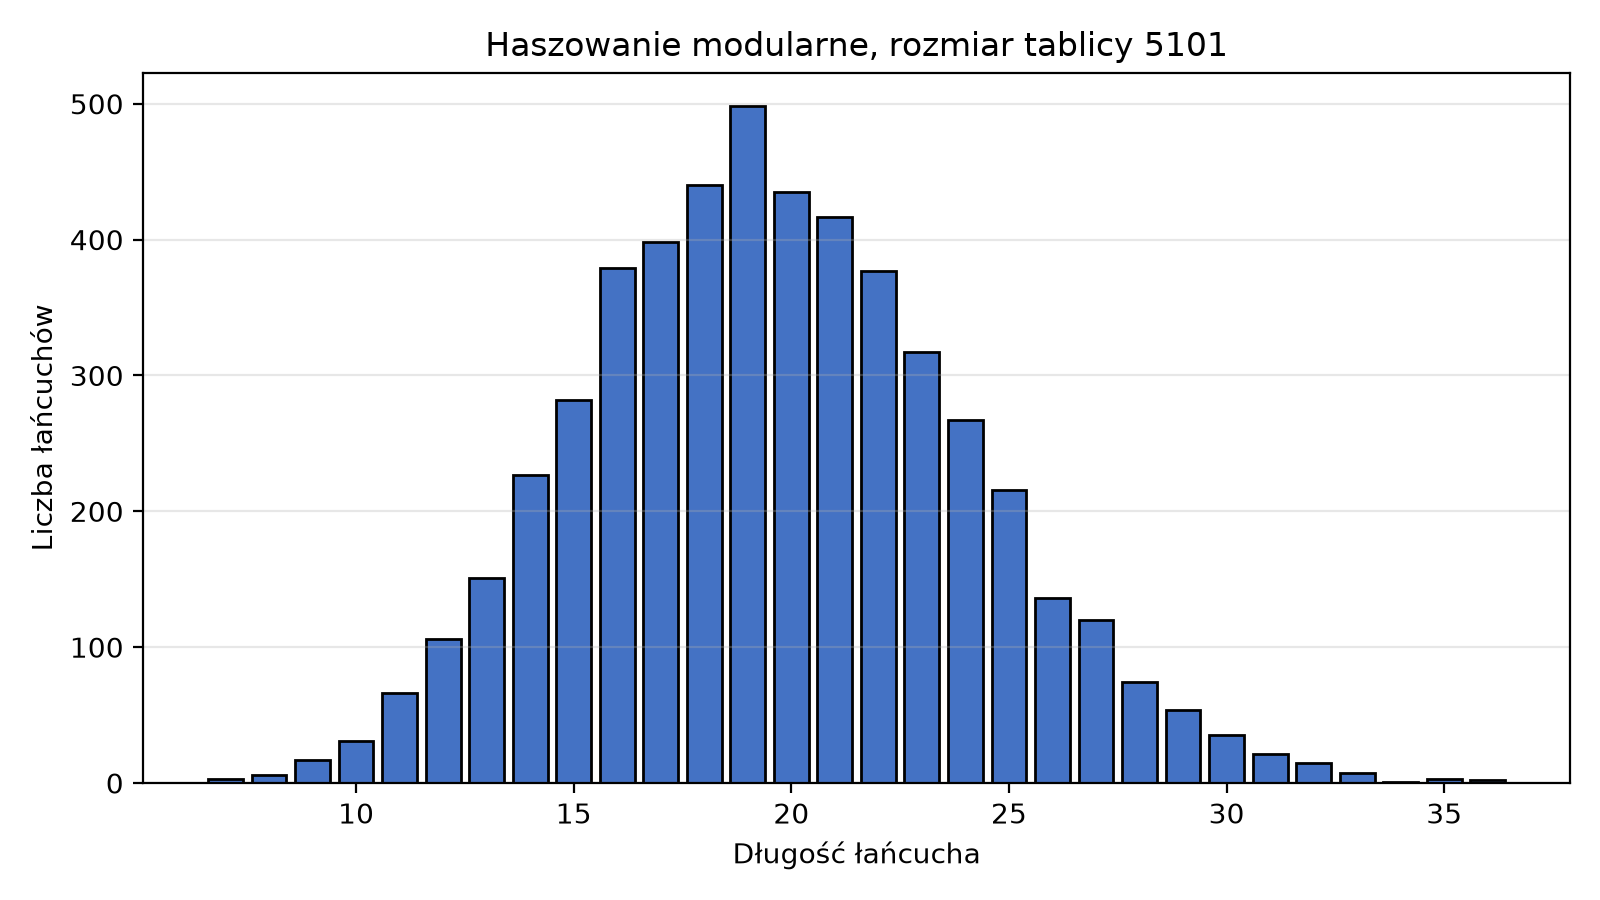
\includegraphics[width=\linewidth]{images/task2_modular_5101.png}
        \caption{Modularne, $m=5101$.}
    \end{subfigure}
    \hfill
    \begin{subfigure}{0.48\textwidth}
        \centering
        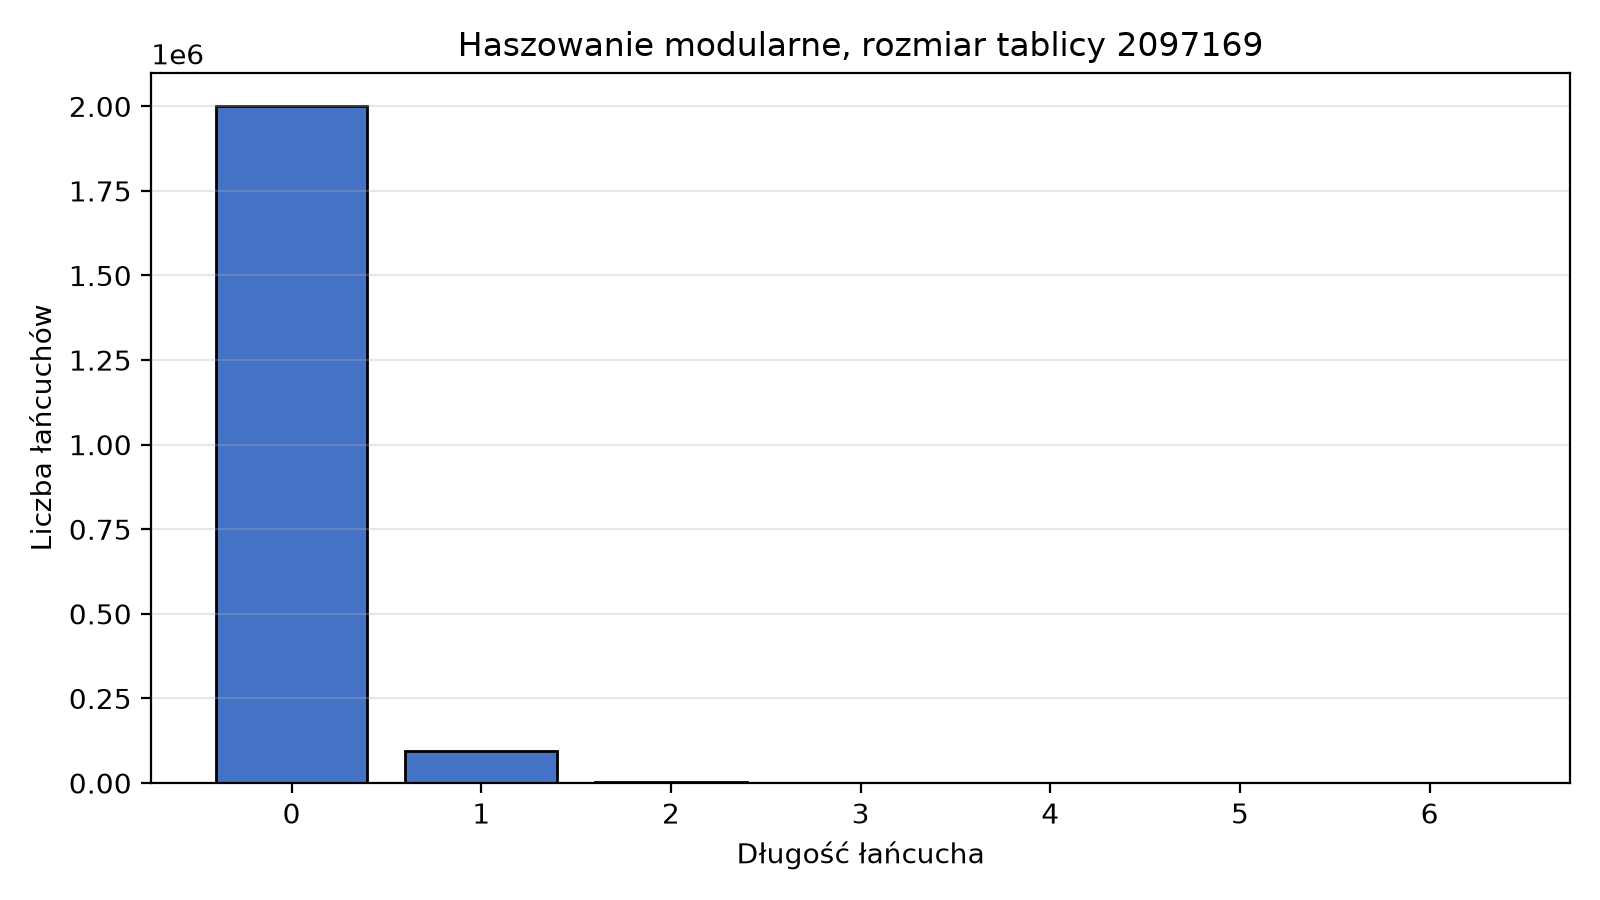
\includegraphics[width=\linewidth]{images/task2_modular_2097169.png}
        \caption{Modularne, $m=2097169$.}
    \end{subfigure}

    \begin{subfigure}{0.48\textwidth}
        \centering
        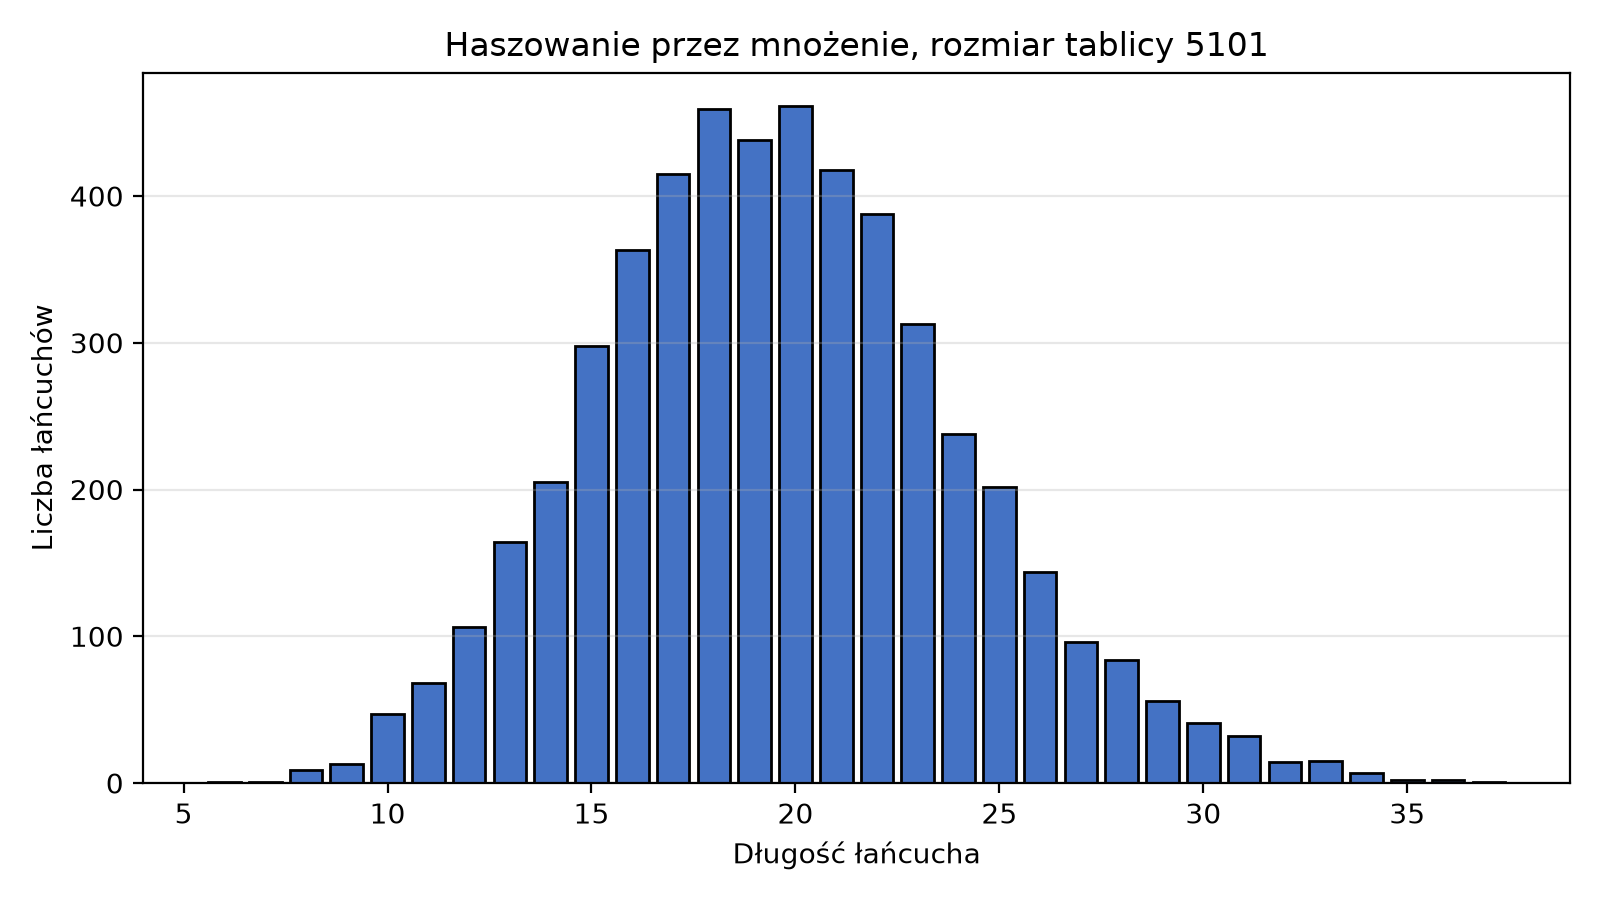
\includegraphics[width=\linewidth]{images/task2_multiplicative_5101.png}
        \caption{Przez mnożenie, $m=5101$.}
    \end{subfigure}
    \hfill
    \begin{subfigure}{0.48\textwidth}
        \centering
        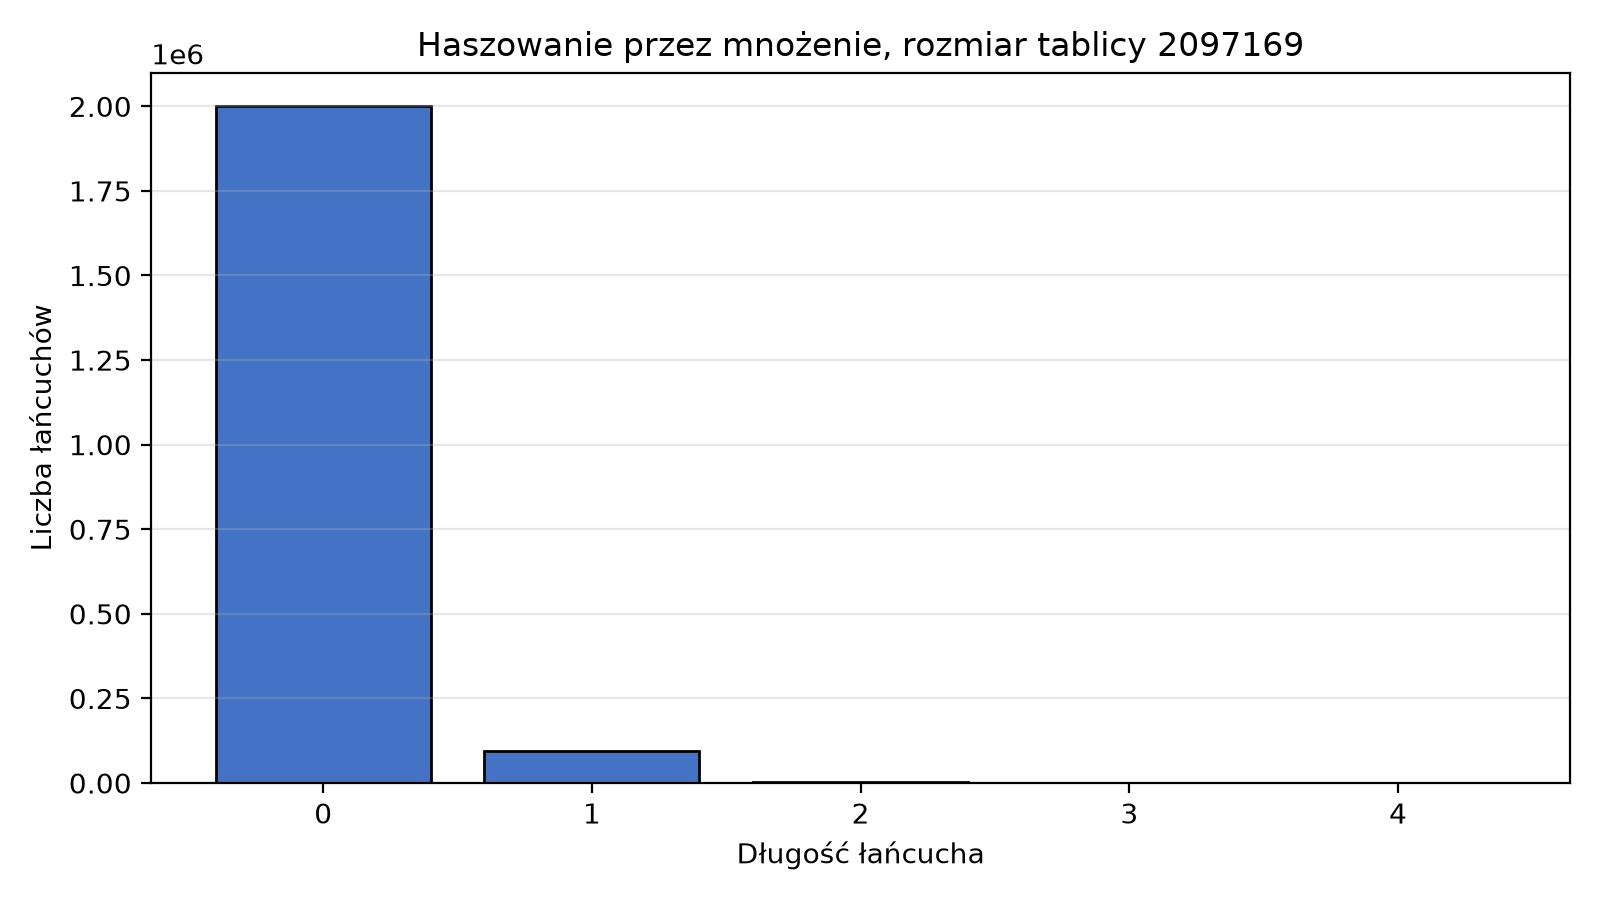
\includegraphics[width=\linewidth]{images/task2_multiplicative_2097169.png}
        \caption{Przez mnożenie, $m=2097169$.}
    \end{subfigure}
    \caption{Liczba łańcuchów w zależności od ich długości.}
    \label{fig:task2-chain-lengths}
\end{figure}

\noindent \textbf{Komentarz (a.k.a. wnioski): }
Dla rozmiaru 5101 współczynnik zapełnienia jest większy, więc łańcuchy są dłuższe. Dla rozmiaru 2097169 większość łańcuchów ma długość 0, czyli są puste. Oba funkcje haszujące dają podobne wyniki.

\newpage 

\subsection{Zadanie 3}
Proszę porównać czas wyszukania $100\_000$ elementów w zależności od: rozmiaru tablicy mieszającej,
użytej funkcji mieszającej. Dla haszowania przez mnożenie proszę zaproponować samemu dwie 
wartości stałej $A$. Proszę skomentować uzyskane wyniki.

%---------------------------------------------------------
% Please, use this tool: https://www.tablesgenerator.com/#
%---------------------------------------------------------
\begin{table}[h]
\begin{tabular}{|l|l|llll|r|}
\hline
\multirow{3}{*}{Lp.} &
  \multirow{3}{*}{Rozmiar} &
  \multicolumn{4}{c|}{Zmierzony czas [ns]} &
  \multicolumn{1}{l|}{\multirow{3}{*}{$\alpha$}} \\ \cline{3-6}
 &
   &
  \multicolumn{1}{l|}{\multirow{2}{*}{H. modularne}} &
  \multicolumn{3}{c|}{H. przez mnożenie} &
  \multicolumn{1}{l|}{} \\ \cline{4-6}
 &
   &
  \multicolumn{1}{l|}{} &
  \multicolumn{1}{l|}{$A=\frac{\sqrt{5}-1}{2}$} &
  \multicolumn{1}{l|}{$A=0.5$} &
  \multicolumn{1}{l|}{$A=\pi-3$} &
  \multicolumn{1}{l|}{} \\ \hline
1. & 5101   & \multicolumn{1}{l|}{12377492} & \multicolumn{1}{l|}{12736097} & \multicolumn{1}{l|}{3511986648} & \multicolumn{1}{l|}{12665778} & 19.60 \\ \hline
2. & 8297   & \multicolumn{1}{l|}{7886148}  & \multicolumn{1}{l|}{8207782}  & \multicolumn{1}{l|}{6051225161} & \multicolumn{1}{l|}{8183160} & 12.05 \\ \hline
3. & 16493  & \multicolumn{1}{l|}{4679930}  & \multicolumn{1}{l|}{4983189}  & \multicolumn{1}{l|}{6037727999} & \multicolumn{1}{l|}{4986535} & 6.06  \\ \hline
4. & 32909  & \multicolumn{1}{l|}{2896459}  & \multicolumn{1}{l|}{3167319}  & \multicolumn{1}{l|}{6055448284} & \multicolumn{1}{l|}{3156599} & 3.04  \\ \hline
5. & 65651  & \multicolumn{1}{l|}{2038385}  & \multicolumn{1}{l|}{2190818}  & \multicolumn{1}{l|}{6053701646} & \multicolumn{1}{l|}{2189921} & 1.52  \\ \hline
6. & 131111 & \multicolumn{1}{l|}{1401893}  & \multicolumn{1}{l|}{1535696}  & \multicolumn{1}{l|}{6024877193} & \multicolumn{1}{l|}{1524993} & 0.76  \\ \hline
7. & 263023 & \multicolumn{1}{l|}{990095}   & \multicolumn{1}{l|}{1076410}  & \multicolumn{1}{l|}{6025884460} & \multicolumn{1}{l|}{1071948} & 0.38  \\ \hline
\end{tabular}
\caption{Tabela pokazuje, jak zmienia się czas wyszukania $100\_000$ elementów w tablicy 
mieszającej w zależności od użytej funkcji mieszającej i rozmiaru tej tablicy.}
\end{table}

\noindent \textbf{Komentarz (a.k.a. wnioski):}
Czasy dla wartości A = $\frac{\sqrt{5}-1}{2}$ oraz A = $\pi-3$ są bardzo zbliżone,
ponieważ wzięta została liczba niewymierna. Wartości czasowe dla hashowania
modularnego są również zbliżone do tych dwóch wartości. Natomiast dla A=0.5
czas jest bardzo duży, ponieważ funkcja haszująca źle rozprasza elementy po
tablicy, przez co powstaje dużo kolizji. Dla A = 0.5 zmniejszyłem ilość
repetycji, ponieważ czas był bardzo duży.

\subsection{Zadanie 4*}
Proszę, wykorzystując gotowe oraz własne testy jednostkowe, zweryfikować poprawność
otrzymanego i uzupełnionego kodu.

\noindent \textbf{Uwaga! To, co poniżej, tylko dla tych, którzy się nudzą.}

Proszę zwrócić uwagę na niedoskonałość (wadę) metody testowej
\verb|should_| \verb|CorrectlyAddThreeDifferentElems_WhenHashSizeIsOne()|
w klasie testowej \verb|GeneralHashListChainingTest|. Metoda ta nie nadaje się do ogólnej klasy testowej, ponieważ nie jest niezależna od konkretnej implementacji interfejsu \verb|HashTable|
(czyli narusza ostatnią zasadę SOLID). Proszę zaproponować zmianę.

\noindent \textbf{Krótki opis proponowanej zmiany:} \hl{TODO ------------------}.

\section{Na zakończenie}
To już prawie koniec, ale nie wolno nam zapomnieć, że:
\begin{itemize}
    \item wszystkie zmiany (cały kod źródłowy) muszą trafić do repozytorium;
    \item ostatnioą zmianę (\textit{commit}), przed końcem zajęć, należy oznaczyć tagiem ze znacznikiem czasowym \textbf{CW\_2\_EOT}.
    A~ostatnią zmianę (\textit{commit}) należy oznaczyć tagiem ze znacznikiem czasowym \textbf{CW\_2\_FINAL};
    \item końcową wersja tego dokumentu (PDF) należy umiecić w ISOD-zie.
\end{itemize}



\end{document}
